% pi.tex
%
%

% R Chandrasekhar
% Department of Mathematics and Statistics
% Curtin University of Technology (CUT)
% R.Chandrasekhar@curtin.edu.au
% First written: 14 Jan 04
% Last revised : 17 Feb 04
% Last revised : 18 Feb 04
% Last revised : 19 Feb 04
% Last revised : 20 Feb 04
% Last revised : 21 Feb 04
%

\documentclass[11pt,a4paper,onecolumn]{article}
%
\usepackage[top=25.4mm,bottom=25.4mm,left=25.4mm,right=25.4mm]{geometry}
\usepackage{cite}
\usepackage{url}
\usepackage{amsmath}
\usepackage{hevea}
\usepackage{textcomp}
\usepackage[dvipsnames]{color}
\usepackage[%
backref,%
colorlinks=true,%
linkcolor=magenta,%
urlcolor=blue,%
citecolor=red,%
filecolor=cyan%
]
{hyperref} % LAST package to be loaded
%
\newenvironment{exercise}{\color [named]{RawSienna} \let \parsave=\parindent%
\setlength{\parindent}{0pt} \sffamily Exercise: }%
{\setlength{\parindent}{\parsave}}
%
\newenvironment{edbox}[1]{\let \parsave=\parindent%
\setlength{\parindent}{0pt}%
\vspace{\parsep}\fbox%
{\parbox{\textwidth}{\vspace{\parsep}#1}}}%
{\vspace{\parsep}\setlength{\parindent}{\parsave}}
%
\newcommand{\maple}{Maple\textsuperscript{\textregistered}}
\newcommand{\map}{Maple}
\newcommand{\maps}{Maple }
%
\input{/home/chandra/LaTeX/tex/PDFPreamble}
%
\begin{document}
%
\input{/home/chandra/LaTeX/tex/GraphicsEPSPDF}
%
\title{Important Numbers and Number Patterns: Pi%
\thanks{This is part of the unit Engineering Mathematics 110, Semester 1, 2004,  at Curtin University of Technology.  The PDF and HTML versions of this document are fully hyperlinked.  Symbol fonts should be enabled on your browser for the HTML version to be displayed correctly.  Otherwise, please use the PDF version.}}
\author{R (Chandra) Chandrasekhar\\
Department of Mathematics and Statistics\\
Curtin University of Technology\\
Room: 314-456\\
Phone: 9266-7623\\
e-mail: \href{mailto:R.Chandrasekhar@curtin.edu.au}%
{\texttt{R.Chandrasekhar@curtin.edu.au}}}
\date{17 February 2004}
%
\maketitle
%
\section{Introduction}

It has been said that% 
%
\begin{equation} 
e^{i\pi} + 1 = 0 
\end{equation}
%
is the most poetic of all mathematical equations because it embodies
the five most important mathematical symbols in one expression.  It is a special case of Euler's formula%
%
\begin{equation}
e^{i\theta} = \cos\theta + i \sin\theta
\end{equation}
%
that relates the exponential and trigonometric functions.

Pi, written as the lowercase Greek letter, $\pi$, is the most famous of
all numbers.  It is the ratio of the circumference of a circle to its
diameter.  The second most famous number $e$ is the base of the natural
logarithms.  The symbol $i$ satisfies $i^2 = -1$, and although it
represents imaginary numbers, its applications in science and
engineering are very real indeed.  Zero and one are familiar from
arithmetic.  They are simple numbers with profound consequences: the
world of digital computers and communications has its foundations in
symbols of zeros and ones.

Other mathematically important numbers include the golden ratio $\phi$,
Euler's constant $\gamma$, and the Feigenbaum number $\delta$. 
Important and useful number patterns include Pascal's Triangle and the
Fibonacci Sequence.

In this series of lectures, we will look at some important numbers, and
number patterns, beginning with $\pi$.

\section{Why is Pi Important?}

It is clear that in day-to-day life, we need to measure lengths, areas, and volumes.  The number $\pi$ enters naturally into the formulae for these measurements for the circle, cylinder and the sphere.  But, surely, this cannot be the only reason why $\pi$ is pre-eminent among numbers.

\subsection{Radians, Trigonometric Functions, and Pi}

Although degrees are generally used to measure angles with a
protractor, the number of degrees in one revolution, or a full  circle,
is an arbitrary number: 360, which most likely has its origins in the
approximate number of days in a year, as determined by the ancient
Babylonians.

A less arbitrary measure of an angle was required for serious
mathematics.  You may recall by looking at Figure~\ref{fig:radians} that
an angle $\theta$ may also be measured in \emph{radians,} as the ratio
of the arc length $s$ subtended at the circumference of a circle, to
the radius $r$ of the circle:
%
\begin{equation}
\theta = \frac{s}{r}
\end{equation}  

%
%------------ Start of Radian Figure ------------
%
\begin{figure}
\begin{center}
\begin{tabular}{c}
\resizebox{0.3\textwidth}{!}%
{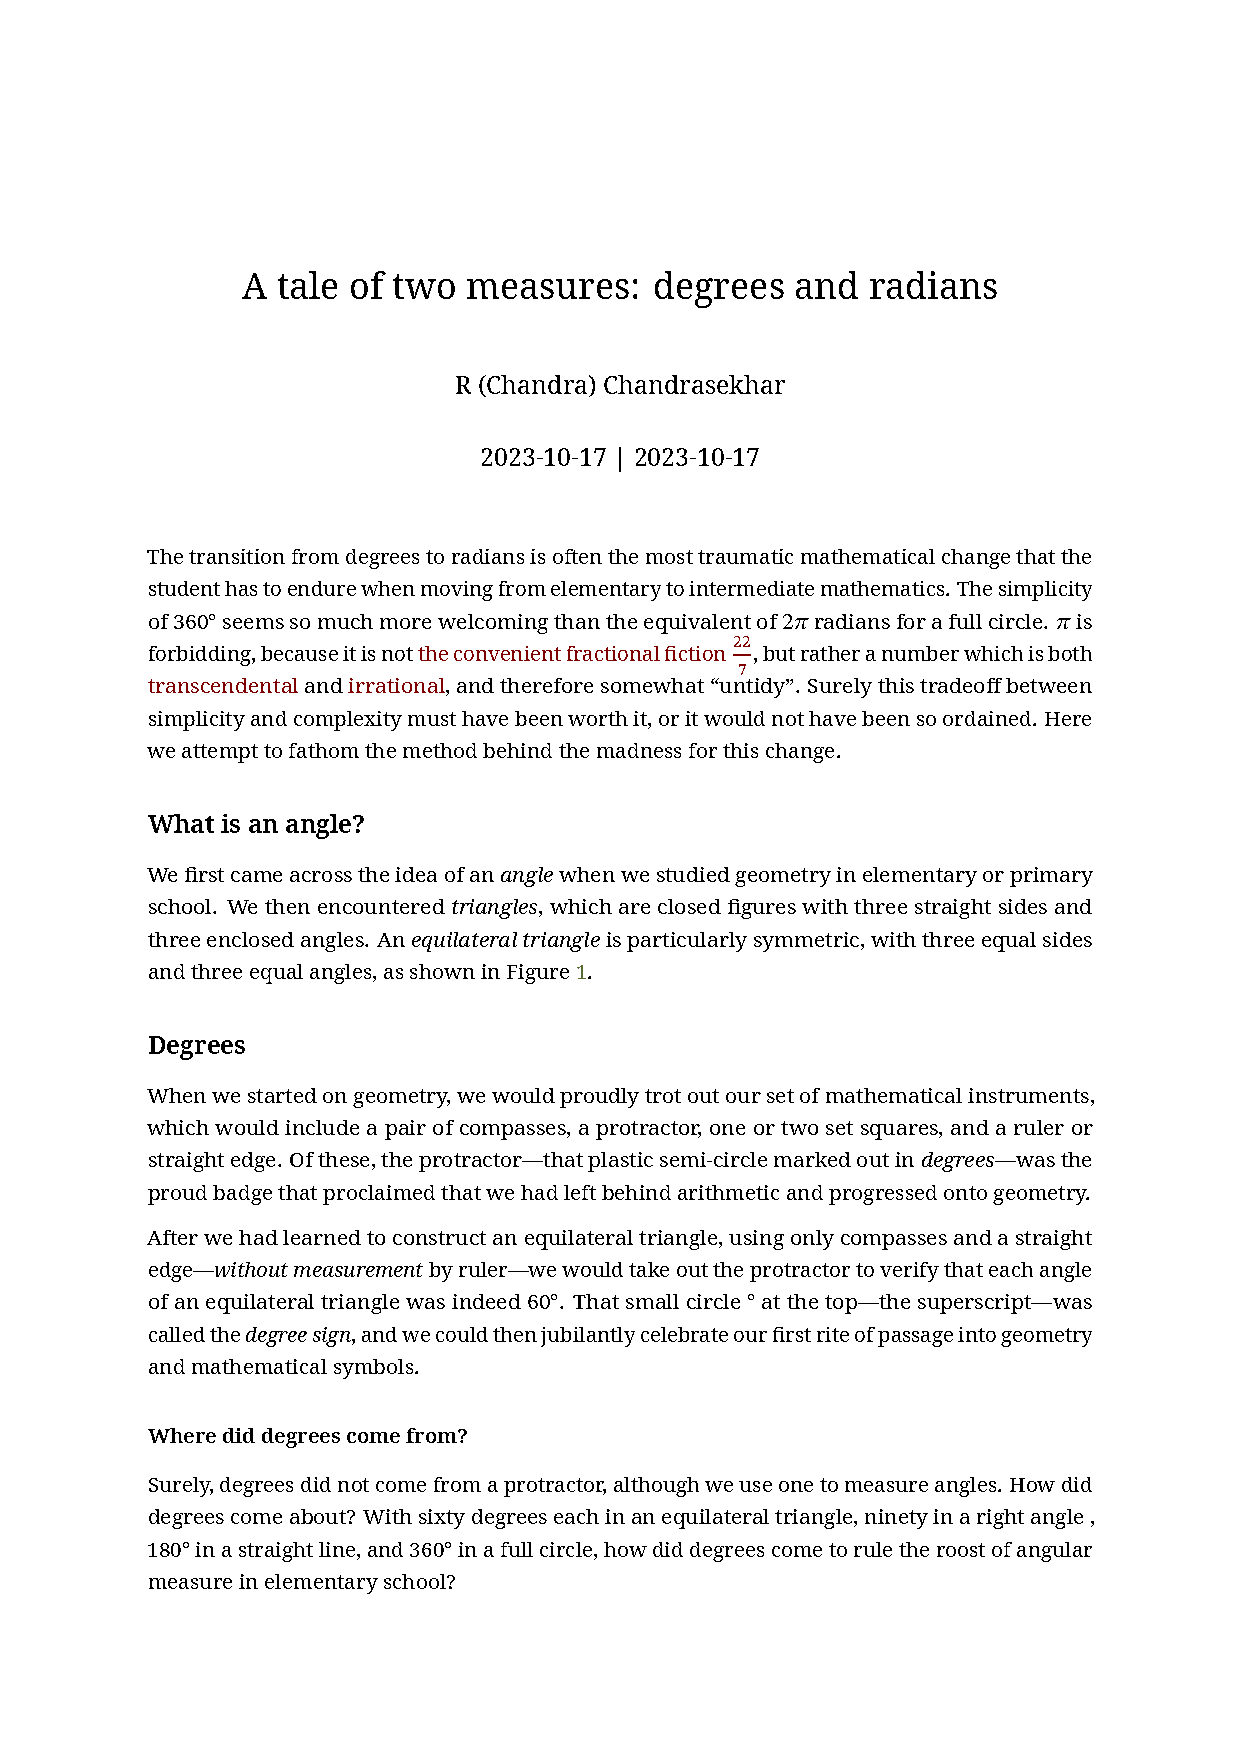
\includegraphics{./graphics/radians}}
\end{tabular}
\end{center}
\caption{\small Radian measure is a normalized, less arbitrary way of measuring angles than degrees.  The angle $\theta$ subtended at the centre of a circle of radius $r$ by an arc of length $s$ is defined to $\theta = \frac{s}{r}$ radians.}
\label{fig:radians}
\end{figure}
%
%------------ End of Radian Figure ------------
%


The ``unit'' radians is not really a unit, though.  Being the ratio of two lengths, it possesses no dimensions in the sense of Physics.  Since the circumference of a circle of radius $r$ is $2\pi r$, one full revolution of 360$^{\circ}$ is actually $2\pi$ radians.  Therefore, the number $\pi$ very naturally enters \emph{angular measure} in radians, and this is one of the principal reasons for its importance.

When trigonometric functions like $\sin x$ are differentiated or integrated, the variable $x$, representing the angle, must be measured in radians.  Moreover, when oscillatory phenomena, whether of water or electricity or light, are studied in the physical sciences and engineering, trigonometric functions usually form part of the solution.  The importance of $\pi$ is therefore entrenched in the importance of trigonometric functions and radian measure, in solving a variety of physical problems.

\subsection{Pi is Irrational and Transcendental}

Pi is not only important, it is also tantalizing.  It is like a
beautiful butterfly that cannot be caught.  It is not a rational
number, which means that it cannot be expressed as the ratio of two
whole numbers, the denominator being non-zero.  Its decimal
representation is neither finite nor does it contain a recurring
segment.  It is also not the root to any polynomial equation whose
coefficients are integers or rational numbers.  This earns for $\pi$
the rather exalted title of a transcendental number, which must also be
irrational by definition.

The unpredictability of successive decimal places of $\pi$ has
enchanted mathematicians and still continues to engross them.  Pi has
been calculated to an unprecedented number of decimal places, and such
a quest is certainly driven not by practical necessity but possibly by
the need for aesthetic satisfaction.

\subsection{Geometry, Algebra, Probability, Limit and Convergence}

We use pictures and words to communicate.  In mathematics,
\emph{geometry} corresponds to pictures, and \emph{algebra} to words. 
The interplay between geometry and algebra has been responsible for
many mathematical advances.  For example, the development of co-ordinate
geometry laid the foundations for calculus.

The search for increasingly more accurate values for $\pi$ has resulted
in many approaches to solve the problem.  Geometric and algebraic
approaches to estimate $\pi$ have both borne fruit.  Interestingly,
$\pi$ may also be estimated by repeatedly performing a random, or
probabilistic, experiment, whose precise outcome cannot be predicted,
but whose average behaviour may be estimated.  Such an experiment is
called a \emph{Monte Carlo} simulation.  Thus the quest for $\pi$
brings together geometry, algebra and probabilistic simulation.

Two of the most important ideas in calculus are those of a \emph{limit}
and of \emph{convergence}.  We shall become acquainted with both as we
find out how $\pi$ may be estimated by these three approaches.

\section{The Method of Archimedes}\label{sec:archi}

Archimedes of Syracuse was one of the greatest mathematicians the world
has known.  By today's standards, he would be called a mathematician,
physicist and engineer, all rolled into one.  He is perhaps most famous
for running out of his bathtub naked exclaiming ``Eureka'' (Greek for
``I have found it'') oblivious of those around him.  The principle that
he had then discovered, that the upthrust on a body submerged in a
fluid is equal to the weight of fluid displaced, is known as
Archimedes' Principle.

Among the many accomplishments of Archimedes is his method for estimating $\pi$, which was the best approximation for almost 1900 years.  What is even more remarkable is that Archimedes made his discovery without the benefit of either  trigonometry or decimal (positional) notation.  His method is also an excellent geometrical illustration of the idea of a limit, with which he was doubtless familiar. It is known that Archimedes was familiar with what we now know as integral calculus, and it is possible that he may have anticipated differential calculus as well. 

Archimedes realized that when a circle is inscribed by a regular
polygon with $n$ sides and circumscribed by a regular polygon with the
same $n$ sides, the circumference of the circle must lie between the
perimeter of the inscribed polygon (limit from below) and the
circumscribed polygon (limit from above).

You may recall that if the limit from below exists, and if the limit
from above exists, and if they are both equal, the limit itself exists,
and is equal to this unique value.

Archimedes started with regular hexagons and successively doubled the
number of sides until he had the circle sandwiched between two
96-gons.  The principle of the method is clearly seen in
Figure~\ref{fig:archi}.
%
% ---------- Start of Archimedes' Method ------------
%
\begin{figure}
\begin{center}
\begin{tabular}{ccc}
\resizebox{0.3\textwidth}{!}%
{\includegraphics{./graphics/archimedes6}} &
\resizebox{0.3\textwidth}{!}%
{\includegraphics{./graphics/archimedes12}} & \resizebox{0.3\textwidth}{!}%
{\includegraphics{./graphics/archimedes24}} \\
$n = 6$ & $n = 12$ & $n = 24$\\
$3.000 < \pi < 3.464$ & $3.105 < \pi < 3.215$ & $3.132 < \pi < 3.159$ \\
\end{tabular}
\end{center}
\caption{\small Illustration of the method used by Archimedes to estimate $\pi$.  The perimeter of the circle is bounded from below by the perimeter of the blue inscribed regular polygon, and bounded from above by the green circumscribed regular polygon.  Archimedes started out with the number of sides, $n = 6$, and stopped at $n = 96$, after four doublings.  Note that with $n = 24$ it is already becoming difficult to distinguish the three figures.}
\label{fig:archi}
\end{figure}
%
% ---------- End of Archimedes' Method ------------
%



We will cheat a little and use trigonometry to derive the perimeters of
the inscribed and circumscribed polygons.  For a polygon of side $n$,
the angle subtended by the any one side at the centre of the circle is
$\frac{2\pi}{n}$.  The half-angle $\theta$ subtended by one side is
therefore $\theta = \frac{\pi}{n}$.  If the radius of the circle is
$r$, the length of one side of the inscribed  polygon is
%
\begin{equation}
s_{i} = 2r\sin\theta
\label{eqn:inpoly}
\end{equation}
%
and likewise, the length of one side of the circumscribed polygon is 
\begin{equation}
s_{c} = 2r\tan\theta
\label{eqn:circumpoly}
\end{equation}

Figure~\ref{fig:sintan} illustrates in one picture what equations~(\ref{eqn:inpoly}) and (\ref{eqn:circumpoly}) state in ``words''.

%
% ---------- Start of sintan figure ------------
%
\begin{figure}
\begin{center}
\begin{tabular}{c}
\resizebox{0.5\textwidth}{!}%
{\includegraphics{./graphics/sintan}}
\end{tabular}
\end{center}
\caption{\small A sector of a circle and parts of the inscribed and
circumscribed polygons are shown above.  The half-angle at the centre
is $\theta = \frac{\pi}{n}$ and the semi-lengths of the sides of
the inscribed and circumscribed polygons are $r\sin\theta$ and
$r\tan\theta$ respectively.} \label{fig:sintan} \end{figure}
%
% ---------- End of sintan figure ------------
%


The circumference of the circle $C = 2\pi r$ is bounded by the perimeters of these two polygons giving us the inequality
%
\begin{equation}
\begin{array}{c}
ns_i < 2\pi r < ns_c \\
2nr\sin\theta < 2\pi r < 2nr\tan\theta \\
n\sin\theta < \pi < n\tan\theta
\end{array}\label{eqn:sintan}
\end{equation}
%

If the number of sides is doubled, $\theta$ is halved, $n$ is doubled, and the equation~(\ref{eqn:sintan}) becomes
%
\begin{equation}
2n\sin\frac{\theta}{2} < \pi < 2n\tan\frac{\theta}{2}
\end{equation}
%
and if the doubling is done $k$ times, we have
%
\begin{equation}
2^{k}n\sin\frac{\theta}{2^{k}} < \pi < 2^{k}n\tan\frac{\theta}{2^{k}}
\label{eqn:sintank}
\end{equation}
%

By making $k$ sufficiently large, we could tighten the bounds on $\pi$ and approximate it arbitrarily closely.  However, if you looked closely at equation~(\ref{eqn:sintank}) and bear in mind that $\theta = \frac{\pi}{n}$ it seems like we have cheated again because equation ~(\ref{eqn:sintank}) really states%
%
\begin{equation}
2^{k}n\sin\frac{\pi}{2^{k}n} < \pi < 2^{k}n\tan\frac{\pi}{2^{k}n}
\label{eqn:sintanpi}
\end{equation}
%

The way out of the circularity into which we have landed is to invoke
the Theorem of Pythagoras and the half-angle formulae, which are
independent of any estimates of $\pi$, but which rely on the roots of
polynomial equations.  The following exercise shows how to go about
this.

\begin{edbox}{%
\begin{exercise}{Estimating $\pi$ using half angle formulae iteratively\\}

In this exercise, you will estimate $\pi$, using the method of
Archimedes as the basis, but employing trigonometric identities to
simplify the work.  This is an iterative exercise which you may try out
with paper and pencil, or with a calculator, or using \maple, the last
of which is recommended.\\

Let $n$ be the number of sides of the regular polygons that inscribe
and circumscribe a circle.  Also, let $\theta = \frac{\pi}{n}$ be the
half-angle subtended at the centre by one side.  We have already shown
that after $k$ doublings of the original number of sides,
%
\begin{equation*}
2^{k}n\sin\frac{\theta}{2^{k}} < \pi < 2^{k}n\tan\frac{\theta}{2^{k}}
\end{equation*}
%
\begin{enumerate}
\item Set $n = 6$, $\theta = \frac{\pi}{6}$, and $k = 0$.  Note that $\sin\theta = \frac{1}{2}$, $\cos\theta = \frac{\sqrt 3}{2}$, and $\tan\theta = \frac{\sqrt 3}{3}$ from Pythagoras' Theorem.

\item Increment $k$ by one. \label{stp:increment}

%$k = 1$, $\frac{\theta}{2^k} = \frac{\theta}{2}$.  

\item Use the half-angle formulae \label{stp:compute}
%
\begin{equation*}
\sin\frac{\theta}{2^k} = %
\left[\frac{1-\cos\left[\frac{\theta}{2^{k-1}}\right]}{2}\right]^%
{\frac{1}{2}}
\end{equation*}
%
\begin{equation*}
\cos\frac{\theta}{2^k} = %
\left[\frac{1+\cos\left[\frac{\theta}{2^{k-1}}\right]}{2}\right]^%
{\frac{1}{2}}
\end{equation*}
%
\begin{equation*}
\tan\frac{\theta}{2^k} = %
\left[\frac{1-\cos\left[\frac{\theta}{2^{k-1}}\right]}%
{1+\cos\left[\frac{\theta}{2^{k-1}}\right]}\right]^{\frac{1}{2}}
\end{equation*}
%
to compute the values of $\sin\frac{\theta}{2^k}$, $\cos\frac{\theta}{2^k}$, and $\tan\frac{\theta}{2^k}$ from the value of $\cos\frac{\theta}{2^{k-1}}$.

\item If $k = 4$ stop; otherwise repeat steps~\ref{stp:increment} to~\ref{stp:compute}.

\item Tabulate your results showing the values of $k$, $2^{k}n\sin\frac{\theta}{2^{k}}$,  $2^{k}n\tan\frac{\theta}{2^{k}}$ and estimate the percentage error of the upper and lower estimates from the last iteration, using the stored value of $\pi$ in your calculator, or \texttt{Pi} in \map.
\end{enumerate}
\end{exercise}}
\end{edbox}

If you found the previous exercise to be demanding, spare a thought for
Archimedes, who attacked and solved the problem without trigonometry,
and without decimals.  He must have devised rational number
approximations to the square roots he encountered, and been careful
enough to keep the rational approximations slightly lower than the
exact values for the lower bound and slightly larger than the exact
values for the upper bound.  As an engineer, you will one day have to
develop the same skills when you perform ``best case'' and ``worst
case'' numerical simulations.

Archimedes reported his result as%
%
\begin{equation}
\begin{array}{c}
\frac{223}{71} < \pi < \frac{220}{70}\\[0.5em]
3\frac{10}{71} < \pi < 3\frac{1}{7}
\end{array}
\end{equation}
%
and most of you will remember this last upper bound as the famous approximation %
\begin{equation}
\pi \approx \frac{22}{7}
\end{equation}
%
from your schooldays.

\section{Gregory-Leibniz Series}\label{sec:gregleib}

It must be obvious by now that trigonometry and the number $\pi$ are
inextricably entwined.  The quest for $\pi$ continued to fascinate
mathematicians in the centuries after Archimedes.  This time though,
rather than geometric iteration, sums of successive terms were used to
approximate $\pi$.

For our purposes, a \emph{sequence} is an \emph{ordered} procession of
numbers, and a \emph{series} is a sum of successive terms that obey
some specific rule.  If the summation stops at some particular term, we
have a \emph{partial sum}; if the summation goes on indefinitely, we
have an \emph{infinite series.}  If this infinite sum approaches ever
closer to a finite value, the series is said to \emph{converge.}  To
see what all this means in practice, let us look at the Gregory-Leibniz
series.

James Gregory was the first Professor of Mathematics at the University
of Edinburgh and in 1671, he published the series now known by his
name.  Rather than draw Gregory's formula out of a hat, we will sketch its derivation, and show its origins in integral calculus.  Gregory found that: %
%
\begin{equation}
\int_{0}^{x}\frac{1}{1+ t^2}dt = \arctan{x}
\label{eqn:invtan}
\end{equation}

This integral should be familiar to you.  If it is not, try substituting $t = \tan \theta$: %
\[
\begin{array}{rcl}
t & = & \tan \theta \quad \mbox{ which gives} \\
\displaystyle \frac{dt}{d\theta} & = & \displaystyle \frac{d}{d\theta}\left[ \tan \theta \right] \\
& = & \sec^2 \theta \\
& = & 1 + \tan^2 \theta \\
& = & 1 + t^2\\
\mbox{Therefore}\quad\frac{1}{1 + t^2}dt & = & d\theta
\end{array}
\]

The integral of equation~(\ref{eqn:invtan}) now becomes%
%
\begin{equation}
\begin{array}{rcl}
\displaystyle \int_{0}^{x}\frac{1}{1+ t^2}dt %
& = & \displaystyle \int_{\arctan0}^{\arctan x} d\theta\\[1em]
& = & \big[ \theta\big]^{\arctan x}_{\arctan0} \\[1em]
& = & \arctan x
\label{eqn:right}
\end{array}
\end{equation}

This takes care of the right hand side of equation~(\ref{eqn:invtan}).  If we performed long division on the left hand side of the same equation, we get %
\begin{equation}
\begin{array}{rcl}
\displaystyle \int_{0}^{x}\frac{1}{1+ t^2}dt %
& = & \displaystyle \int_{0}^{x}%
\left[ 1 - t^2 + t^4 - t^6 +\dots \right] dt \\[1em]
& = & \displaystyle \left[ t - \frac{t^3}{3} + \frac{t^5}{5} - \frac{t^7}{7}+ \dots \right]_{0}^{x}\\[1em]
& = & \displaystyle x - \frac{x^3}{3} + \frac{x^5}{5} - \frac{x^7}{7}+ \dots
\label{eqn:left}
\end{array}
\end{equation}

Using equations~(\ref{eqn:right}) and (\ref{eqn:left}), we get the Gregory series
%
\begin{equation}
\arctan x = x - \frac{x^3}{3} + \frac{x^5}{5} - \frac{x^7}{7} + \dots
\label{eqn:gregory}
\end{equation}
%
Notice that it is only a small step from here to substitute $x = 1$ to
get the equation %
%
\begin{equation}
\begin{array}{ccccc}
\arctan 1 & = & \frac{\pi}{4} & = & 1 - \frac{1}{3} + \frac{1}{5} - \frac{1}{7} + \dots \\[0.5em]
&  & \pi & = & 4(1 - \frac{1}{3} + \frac{1}{5} - \frac{1}{7} + \dots)
\end{array}
\label{eqn:leibniz}
\end{equation}

Strangely, Gregory did not publish the special case of
equation~(\ref{eqn:leibniz}), and it was Gottfried Wilhelm Leibniz who
discovered both equations~(\ref{eqn:gregory}) and (\ref{eqn:leibniz})
in 1674, and published them in 1682.  Thus the dual names by which these
series are known.  

It is noteworthy that equation~(\ref{eqn:leibniz}) was the
first infinite series ever found for $\pi$.  However, it converges rather slowly, and one needs many terms before a reasonable approximation emerges.

Over the last 350 years, by far the most effort has been expended in
discovering series that \emph{converge rapidly} to $\pi$, so that even
a partial sum of only a few terms will provide an accurate estimate of
$\pi$.

We wrap up this section with a selection of formulae from famous mathematicians who have bequeathed other series for calculating $\pi$.

Newton used the binomial theorem to derive: %
%
\begin{equation}
\begin{array}{lcl}
\arcsin x & = & x + \frac{1}{2}\frac{x^3}{3} + %
\frac{1\cdot 3}{2\cdot 4}\frac{x^5}{5} + \dots \\[0.5em]
%\mbox{for which, substituting $x = \frac{1}{2}$ gives} & & \\
\pi & = & 6\left( \frac{1}{2} + \frac{1}{2}\frac{1}{3 \cdot 2^3} + %
\frac{1 \cdot 3}{2 \cdot 4}\frac{1}{5 \cdot 2^5} + \dots\right)
\end{array}
\end{equation}

John Machin gave the formula: %
%
\begin{equation}
\frac{\pi}{4} = 4 \arctan \left[ \frac{1}{5} \right] %
- \arctan \left[ \frac{1}{239} \right]
\end{equation}
%
where $\arctan x$ may be approximated by equation~(\ref{eqn:gregory}).

Karl Friedrich Gauss gave the elegant formula: %
%
\begin{equation}
\frac{\pi}{4} = \arctan \left[\frac{1}{2}\right] + \arctan \left[\frac{1}{5}\right] + \arctan \left[\frac{1}{8}\right]
\label{eqn:gauss}
\end{equation}

which again may be computed using equation~(\ref{eqn:gregory}).

Among the countless formulae for $\pi$ may be mentioned one, due to Srinivasa Ramanujan, which is so \emph{unusual} that one wonders how it was ever derived in the first place: %
%
\begin{equation}
\frac{1}{\pi} = \frac{\sqrt 8}{9801}\sum_{n = 0}^{\infty}%
\frac{(4n)!\left[ 1103 + 26390n \right]}{(n!)^4 396^{4n}}
\end{equation}

We conclude this section with an exercise that explores convergence and gives a practical measure for estimating its rate.

\begin{edbox}{%
\begin{exercise}{Rates of convergence for different formulae for $\pi$ \\}

You will explore the different rates of convergence for four of the  formulae that we have encountered: the Gregory-Leibniz series, Newton's formula, Machin's formula, and Gauss's formula.  Proceed as follows, using \map:%
\begin{enumerate}

\item Write expressions for the general terms for each formula and assign them to four different variables.

\item Write expressions for the sum to $n$ terms for each formula.

\item Compute this sum for $n = 10^k; \, k = 0, 1, \dots , 10$.

\item For each value of $k$, calculate the percentage error in the respective partial sums by subtracting them from $\pi$, dividing by $\pi$, and multiplying by 100.  Use the \maps constant \texttt{Pi} for this. 

\item Plot the percentage error as dependent variable against $\log_{10}n = k$ as dependent variable.  Use semi-log axes.

\item Comment on the different rates of convergence of the four formulae.  If you had to choose a formula, which would you choose, and why?
%
\end{enumerate}
\end{exercise}}
\end{edbox}

\section{Buffon's Needle}\label{sec:buffon}

In the preceding two sections, we have seen the connection between
$\pi$ and geometry, and between $\pi$ and trigonometry.  Such a
relationship is not unexpected, for we may mataphorically say that
$\pi$ has its ``home'' in the circle, and is ``neighbours with''
trigonometric functions, which are also called \emph{circular
functions.}  But how indeed does $\pi$ enter the domain of
probability?

Georges Louis Leclerc Comte de Buffon was a French naturalist of the
eighteenth century, who is probably most well-remembered for proposing
and solving the problem that goes by his name.  It is a  probabilistic
method for determining the value of $\pi$, and antedates modern
\emph{Monte Carlo} simulations on computers.

Buffon's Needle problem may be posed thus.  Consider a needle of length
$\ell$ that is thrown at random on a floor that has parallel lines
spaced $d > \ell$ apart. What is the probability that the needle will
touch or cross one of the lines?  We may assume that the needle's
position and its orientation, when it lands, are both independent, and
random.

This problem may be solved elegantly using knowledge of trigonometry
and the integral calculus.  First we draw a diagram of how the needle
may fall with respect to a \emph{single} line, as shown in
Figure~\ref{fig:buffon}.  It is important to realize that the analysis
with respect to a single line suffices.  This sort of \emph{problem
abstraction} or \emph{modelling} is an important skill you should
acquire as engineers, because it helps focus on the essentials, and in
the process usually simplifies the solution of the problem.

%
% ----------- Start of Buffon's Needle Figure -----------
%
\begin{figure}
\begin{center}
\begin{tabular}{c}
\resizebox{0.5\textwidth}{!}%
{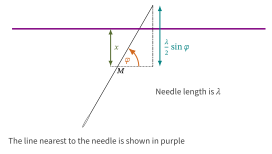
\includegraphics{./graphics/buffon}}
\end{tabular}
\end{center}
\caption{\small Illustration of \emph{problem abstraction} for solving
the problem of Buffon's Needle.  Because the spacing between the
parallel lines $d$ is greater than the length of the needle $\ell$, we
know that the needle can \emph{at most} intersect \emph{one} line.  We
have shown that one line here, and called it the nearest line.  The
perpendicular distance from the centre of the needle to the nearest
parallel line is denoted by $x$.  By relating $x$ to the angle $\phi$
and needle length $\ell$, we derive the condition for intersection or
non-intersection as a simple inequality.}
\label{fig:buffon}
\end{figure}
%
% ----------- End of Buffon's Needle Figure -----------
%

With reference to Figure~\ref{fig:buffon}, let $x$ be the perpendicular
distance from the centre of the needle to the nearest parallel line. 
If the needle makes an angle $\phi$ measured in the conventional sense
with respect to the nearest line, the distance of the tip of the needle
from the centre, in the direction perpendicular to the parallel lines,
is $\frac{1}{2}\ell \sin\phi$.  Clearly, if $x > \frac{1}{2}\ell
\sin\phi$, the needle cannot touch the nearest line.  Therefore the
condition for the needle to touch the nearest line is %
%
\begin{equation}
x \leq \frac{1}{2}\ell \sin\phi
\label{eqn:buffon}
\end{equation}

Because of symmetry, we may restrict our consideration to angles $0
\leq \phi \leq \pi$ and for $0 \leq x \leq \frac{d}{2}$.  We may now
define the space of all events as the rectangle on the $\phi$-$x$ plane
bounded by the lines $x=0$, $\phi = \pi$, $x = \frac{d}{2}$ and $\phi =
0$, as shown in Figure~\ref{fig:buffonspace}.  

The set corresponding to the needle touching or crossing a line is the set of all points for which inequality~(\ref{eqn:buffon}) is satisfied.

%
% ----------- Start of Buffon's Needle Probability Space -----------
%
\begin{figure}
\begin{center}
\begin{tabular}{c}
\resizebox{0.5\textwidth}{!}%
{\includegraphics{./graphics/buffonspace}}
\end{tabular}
\end{center}
\caption{\small Graphical depiction of the event space for the Buffon
Needle experiment.  The area under the curve satisfies the inequality
$x \leq \frac{1}{2}\ell \sin\phi$.  Let this area be called A. We show
in equation~(\ref{eqn:al}) that $A = \ell$.  The universal set is the
rectangle bounded by the $\phi$ and $x$ axes and the lines $x
=\frac{d}{2}$ and $\phi = \pi$ as shown.  Its area is simply $\frac{\pi
d}{2}$.  The probability that the needle will touch or cross one of the
parallel lines is therefore $\frac{A}{\frac{\pi d}{2}}$.  (The values
of $d$ and $\ell$ have been arbitrarily set to 3 and 2 respectively in
this diagram, with no loss of generality.)}
\label{fig:buffonspace}
\end{figure}
%
% ----------- End of Buffon's Needle Figure -----------
%

The area $A$ under the curve in Figure~\ref{fig:buffonspace} is given by%
\begin{equation}
\begin{array}{rcl}
A & = & \displaystyle \frac{1}{2}\ell\int_{0}^{\pi} \sin \phi \, d\phi \\[0.5em]
& = & \left[ -\cos\phi \right]_{0}^{\pi}\\
& = & \frac{1}{2}\ell[2] \\
& = & \ell
\end{array}\label{eqn:al} 
\end{equation}

The probability that the needle touches or crosses a parallel line is therefore equal to %
%
\begin{equation}
\begin{array}{rcl}
P(\ell, d) & = & \displaystyle \left[ \frac{A}{\frac{\pi d}{2}} \right] \\[0.5em]
& = & \displaystyle \left[ \frac{\ell}{\frac{\pi d}{2}}\right ]\\[2em]
& = & \displaystyle \frac{2\ell}{\pi d}
\end{array} 
\end{equation} 

If a probabilistic experiment is repeated independently a great many
times, the relative frequency of the event whose probability we are
trying to measure, approaches the true probability.  Using this
principle, it is possible to simulate Buffon's needle experiment on
computer, calculate the relative frequency, associate it with the
theoretical probability, and thereby derive $\pi$.

Incidentally, the derivation of the probability $P(\ell, d)$ \emph{does}
involve geometry and trigonometry, and the appearance of $\pi$ is not so
inexplicable after all.

\section{The Quest for Ever Greater Precision}\label{sec:precision}

In 1560, $\pi$ was known only to 6 decimal places.  By 1706, it had
been computed to 100 decimal places.  This jumped to 707 by 1874.  In
1947, $\pi$ was known to 808 decimal places.  The advent of computers
meant that by 1957, the number of decimal places had grown to 10,000.
By 1967, this number had climbed up to 500,000.  In 1997, researchers
in Japan computed $\pi$ to a mind-boggling 51.5 \emph{billion} decimal
places.

One may wonder what drives this quest for ever greater precision.  As
we have already observed, it is not driven by practical need.  Because
$\pi$ is ultimately unknowable as a decimal number, it has a mystery to
it.  Each successive attempt to improve the precision to which it is
known, is a quest to tame the untameable.

But apart from aesthetic motives, the decimal expansion of $\pi$ may reveal new knowledge about number sequences, randomness, and how to generate random numbers. 
  
\section{Maple Notes}

In \map, the constant $\pi$ is designated by the mathematical constant \texttt{Pi}, which is therefore a reserved keyword.  In keeping with Maple's philosophy of retaining precision in calculations, typing \texttt{Pi;} at the \maps prompt $[>$ only displays the symbol $\pi$.

What does typing \texttt{pi;} do?  It also simply displays the symbol $\pi$.  The difference between the two may be discovered by typing \texttt{sin(Pi);} which gives the result $0$ whereas typing \texttt{sin(pi);} simply echoes back the expression $\sin(\pi)$.  To be sure, try typing \texttt{beta} and see whether you get $\beta$ echoed.  Evidently, \maps knows its Greek lowercase letters!

If you try to assign a value to \texttt{Pi}, by typing, say, \texttt{Pi := 22/7;} you will get an error message saying that you tried to assign a value to \texttt{Pi} which is protected.

If you want a numerical value for $\pi$ from \map, you need to evaluate the constant by typing \texttt{evalf(Pi);} which gives the number $3.141592654$.  If you wanted $\pi$ to be evaluated to 50 \emph{digits,} not decimal places,  you would type \texttt{evalf(Pi, 50);} and you world see the result to 50 glorious digits.

\maps uses an environment variable called \texttt{Digits} that controls the number of digits when \maps calculates with floating point numbers.  To find the default value of this variable, type \texttt{Digits;}.  Very likely, you saw the answer $10$ which is the default setting.

Now, type \texttt{kernelopts(maxdigits);} and you will see an answer
that depends on your platform.  You may see a number close to
$2^{28}$.  This is the theoretical maximum number of digits that Maple can display.

Now for some questions to ponder about.

How does \maps perform arbitrary precision arithmetic that enables
results to be output, correct to, say, 50 digits?

Also, how does \maps respond so promptly when you type
\texttt{evalf(Pi, 50);}?

What algorithm(s) does \maps use to calculate $\pi$?

Finally, some information about useful Maple-related websites.  \href{http://www.mapleapps.com/}{The Maple Application Center}  is a very useful web site from which to learn about \map.  You should also visit the \href{http://www.maple4students.com/}{Maple Student Center} which contains many resources for students.

Gregory Moore has an
\href{http://www.mapleapps.com/powertools/geom/html/Pi.html}{introductory
web site on $\pi$} using \map.  It is part of the
\href{http://www.mapleapps.com/powertools/geom/geometry.shtml}{PowerTools Geometry} package.

\section{Book References}

There is no prescribed textbook for this series of lectures on important
numbers and number patters.  Accordingly, a rather comprehensive list
of references is given at the end of each set of notes.

The notes for this lecture have been compiled mainly from four books. 
The first is the encyclopaedic source book on $\pi$ by Berggren et
al.~\cite{pi_source}.  It contains a wealth of historical information
and has facsimiles of many original publications or their
translations.  Interestingly, the next two references are written by
engineers.  Beckmann's book~\cite{beck71}, although somewhat dated and
opinionated, gives detailed historical accounts of efforts at computing
$\pi$.  The book by Banks~\cite{banks99} is a delightful, instructive
and entertaining romp through some areas of applied mathematics.  It is
easy to read and  devotes three chapters to famous numbers and number
sequences.  Lastly, the popular book by Blatner~\cite{blat97} is
historically informative and instructive.

\section{Web Resources}

If you are unsure about a mathematical term, or definition, I would
recommend, as first port of call,
\href{http://mathworld.wolfram.com/}{Eric Weisstein's World of
Mathematics}~\cite{mathworld}.  It is a searchable, authoritative and
encyclopaedic web site.  Although Weisstein is himself an astronomer,
his enduring love of Mathematics has resulted in this treasure trove of
mathematical information on the web, from which all can benefit.

The lives of mathematicians have been chronicled at several places on
the Web.  One of the most comprehensive and scholarly---fully
searchable, and with many related links---is
the~\href{http://www-history.mcs.st-andrews.ac.uk/history/index.html}%
{MacTutor History of Mathematics archive}~\cite{mactutor_history}. 

\section{To Probe Further}

If you have in any way been intrigued by what is in these lecture notes,
and you have the time and interest to pursue these ideas further, you
may wish to look at some of the books or web sites discussed in this
section.

The development in Sections~\ref{sec:archi}, \ref{sec:gregleib} and \ref{sec:buffon} follows that of Beckmann~\cite{beck71}.  The numbers quoted in Section~\ref{sec:precision} are from Banks~\cite{banks99}.

A faithful account of how Archimedes used the geometry of his day to
arrive at his estimates of $\pi$ is given in the translation of his
original works by Heath~\cite{heath02}. 
\href{http://itech.fgcu.edu/faculty/clindsey/mhf4404/archimedes/archimedes.html}{Chuck
Lindsey's web site} gives a web-based account of the same. 

The web site by
\href{http://www.math.utah.edu/~alfeld/Archimedes/Archimedes.html}{Peter
Alfeld} is particularly interesting because it has a Java applet that
illustrates the method of Archimedes and allows the user to
progressively change the number of sides in the polygons and view the
corresponding upper and lower limits on $\pi$.

The life of Archimedes makes fascinating reading.  He comes across as the archetypical absent-minded scientist, totally engrossed in his work, oblivious of everything else.  You can find out more about him from one of these web sites~\cite{mactutor_history,golba_archi}.

You may wish to find out more about the formulae for computing $\pi$ at \href{http://mathworld.wolfram.com/PiFormulas.html}{Eric Weisstein's Pi Formulas}.  One particularly interesting formula is that of Wallis: it is composed of an infinite product of rational numbers to yield the irrational number $\pi$.  The book by Blatner~\cite{blat97} gives a brief account of the astounding achievement of the brothers Chudnovsky in developing efficient algorithms for calculating $\pi$. 

There are two web sites with simulations of the Buffon's Needle
experiment. \href{http://www.mste.uiuc.edu/reese/buf
fon/buffon.html}{George Reese's site} has a discussion and simulation
of the experiment.  \href{http://www.angelfire.com/wa/hurben
/buff.html}{Michael Hurben's site} not only has a simulation, but also
tracks and displays how close the estimate of $\pi$ approaches the true
value as the experiment is repeated.

If you wish to explore more about $\pi$, the Fibonacci sequence, and
other numbers, you may want to visit
\href{http://www.mcs.surrey.ac.uk/Person
al/R.Knott/Fibonacci/fibpi.html}{Ron Knott's information-packed site}.

Although $\pi$ is known to more digits than we care to count, such is its allure that the quest for computing $\pi$ is not over yet and programming enthusiasts still have active projects for this purpose~\cite{pi_comp}.

\bibliographystyle{ieeetr}
%
\bibliography{%
/home/chandra/Bibliography/abbrev,%
/home/chandra/Bibliography/pi,%
/home/chandra/Bibliography/piWeb,%
/home/chandra/Bibliography/mathWeb%
}
%
\end{document}
